\documentclass[../main.tex]{subfiles}
\begin{document}
\section{Basic concepts}
This section contains examples and counterexamples about invariants and properties of objects in elementary algebraic geometry (schemes, sheaves, divisors, linear systems etc), morphisms (projective, flat, smooth, \'{e}tale, etc) and behavior of invariants and properties along morphisms (base-change, push-forward, pull-back, etc)
\begin{figure}[h!]
\centering
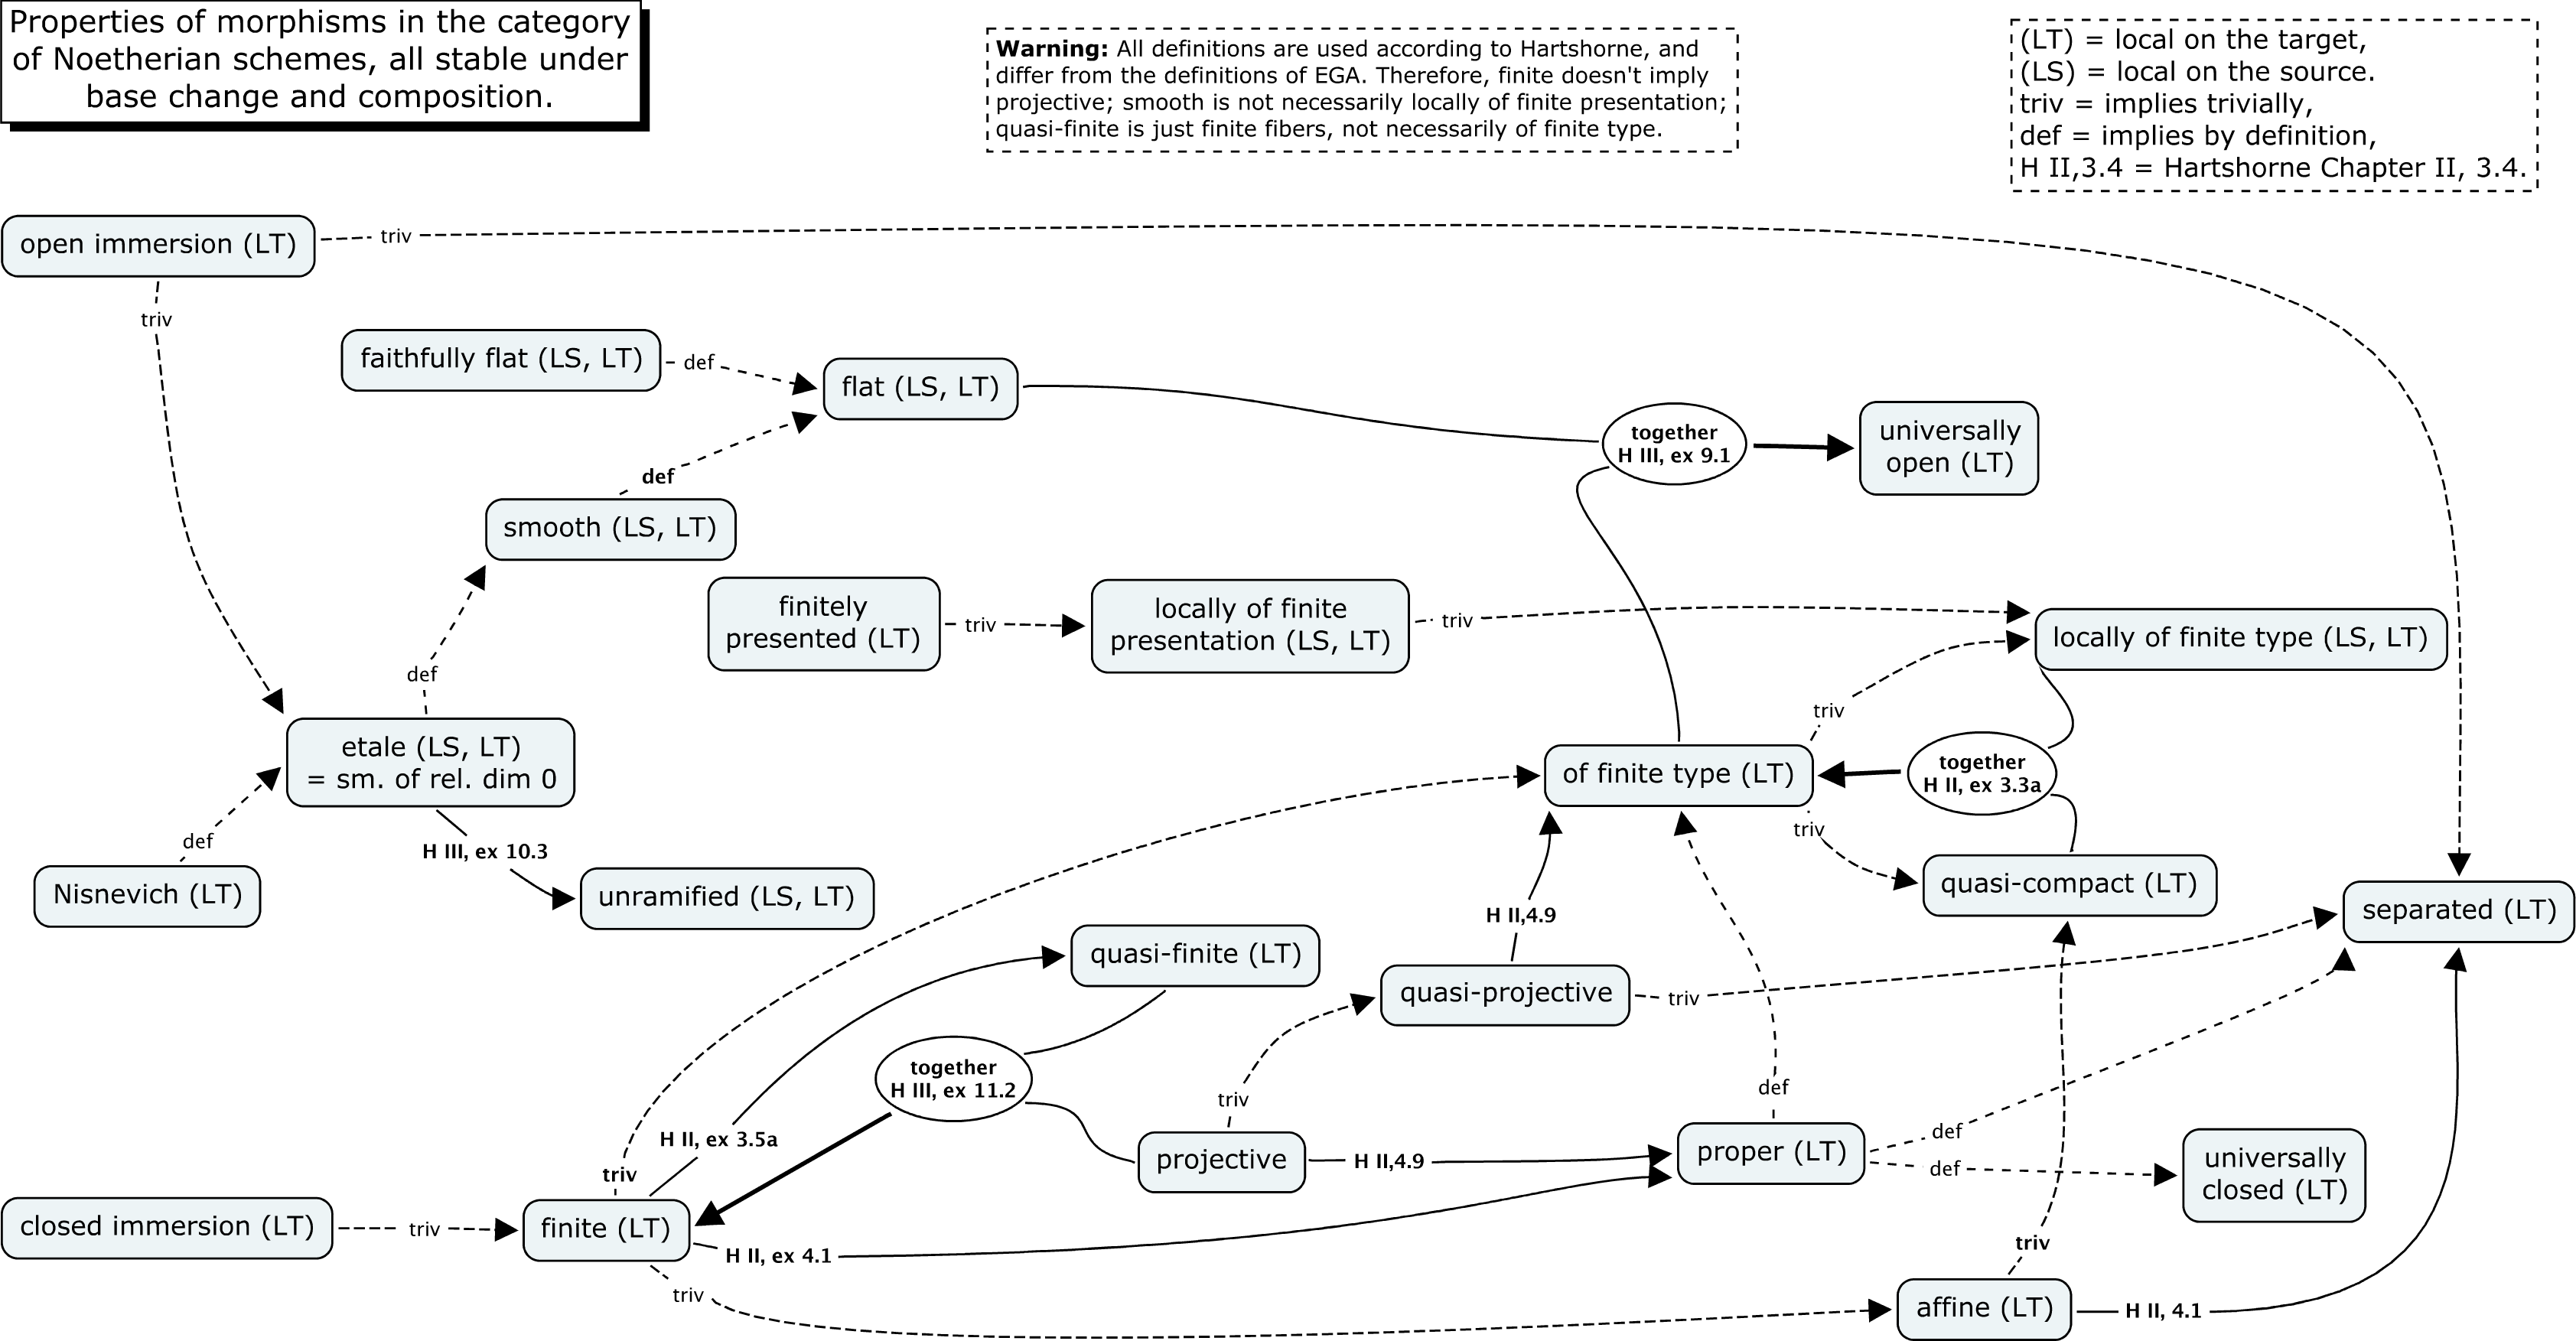
\includegraphics[width=\textwidth]{img/morphisms.png}
\caption{Properties of scheme morphisms. Konrad Voelkel}
\label{fig:Properties of sheme morphims; Konrad Voelkel}
\end{figure}
\end{document}